\appendix

%%%%%%%%%%%%%%%%%%%%%%%%%%%%%%%%%%%%%%%%%%%%%%%%%%%%%%%%%%%%%%%%%%%%%%%%%%%%%%%%%%%%%%%%%%%%%%%%%
%
%
%
%%%%%%%%%%%%%%%%%%%%%%%%%%%%%%%%%%%%%%%%%%%%%%%%%%%%%%%%%%%%%%%%%%%%%%%%%%%%%%%%%%%%%%%%%%%%%%%%%
\clearpage
\onecolumngrid
\section{Supplementary Figures}
\setcounter{figure}{0}
\renewcommand{\thefigure}{SF\arabic{figure}}



% --------------- Dim red time series and free energy profiles
\begin{figure}[h!]
    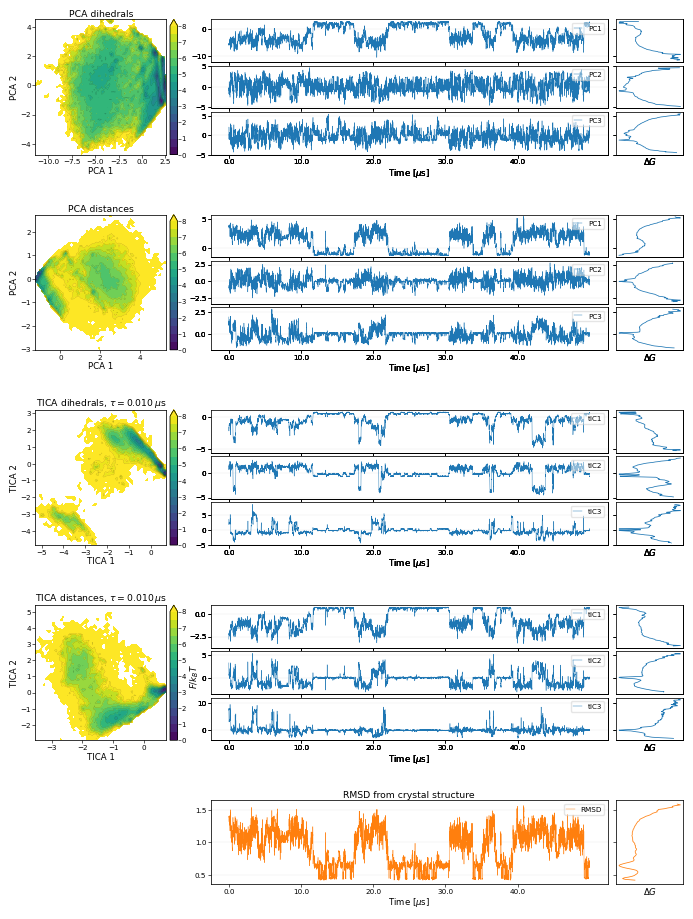
\includegraphics[width=0.8\linewidth]{figures/RMSD_reduced_projection_A4.png}
\caption{\small
\textbf{Reduced-coordinate representations obtained from the four feature–dimensionality-reduction pipelines.}
Rows correspond to PCA dihedrals, PCA contact distances, tICA dihedrals, and tICA contact distances. For each pipeline, the left panel shows the projection of the trajectory onto the first two reduced coordinates. The remaining panels show the time evolution of the first three reduced coordinates during the first $\sim40\,\mu\mathrm{s}$ of simulation together with the corresponding one-dimensional free-energy profiles computed from the full trajectory. The bottom row reports the RMSD from the crystal structure and its free-energy profile for comparison.
}
    \label{suppfig:dimred_figure}
\end{figure}

% ---------------Implied timescales test
\begin{figure*}[ht]
    \centering
    
\includegraphics[width=0.7\linewidth]{figures/implied_timescales_report.pdf}
    \caption{\textit{\small \textbf{Results of the timescale convergence test}:
     First three implied timescales as a function of the MSM lagtime. Colors denote the four combinations of feature set and dimensionality reduction method, while marker styles indicate the number of microstates used in the state-space discretization. 
        The shaded region corresponds to $t_i \leq \tau_{MSM}$, where $t_i$ is the implied timescale and $\tau_{MSM}$ the MSM lagtime. Timescales falling within this region are not resolved by the model, 
        as the associated relaxation process occurs on a timescale shorter than a single Markov-chain transition step.}}
    \label{suppfig:timescales_test}
\end{figure*}
% --------------- MSM connectivity and active population as a function of lag time
\begin{figure}[h!]
    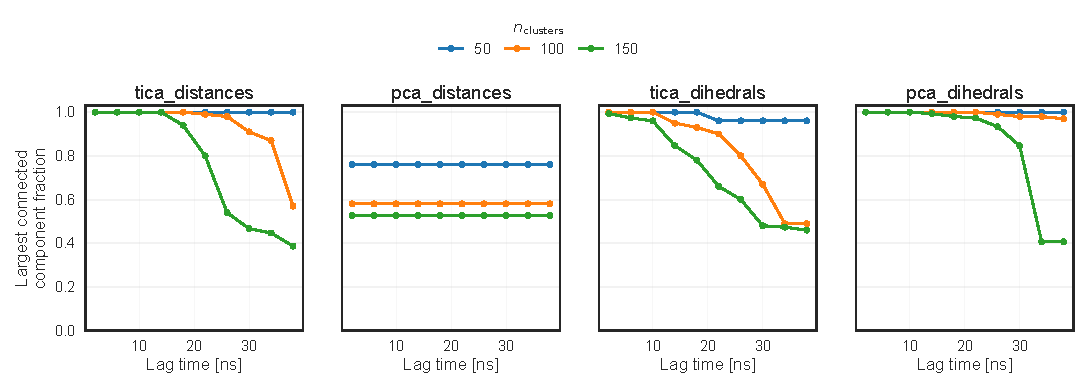
\includegraphics[width=0.7\linewidth]{figures/largest_connected_component_vs_lag.pdf}
    
\includegraphics[width=0.7\linewidth]{figures/active_population_vs_lag.pdf}
    \caption{\small \textbf{MSM connectivity and active population as a function of lag time.}
    Top panel: fraction of microstates in the largest connected component of the MSM as a function of lag time. 
    Bottom panel: fraction of the total equilibrium population contained in the largest connected component of the MSM as a function of lag time}
    \label{suppfig:largest_connected_component_vs_lag}
\end{figure}


% -------------- CK test

\begin{figure}[h!]
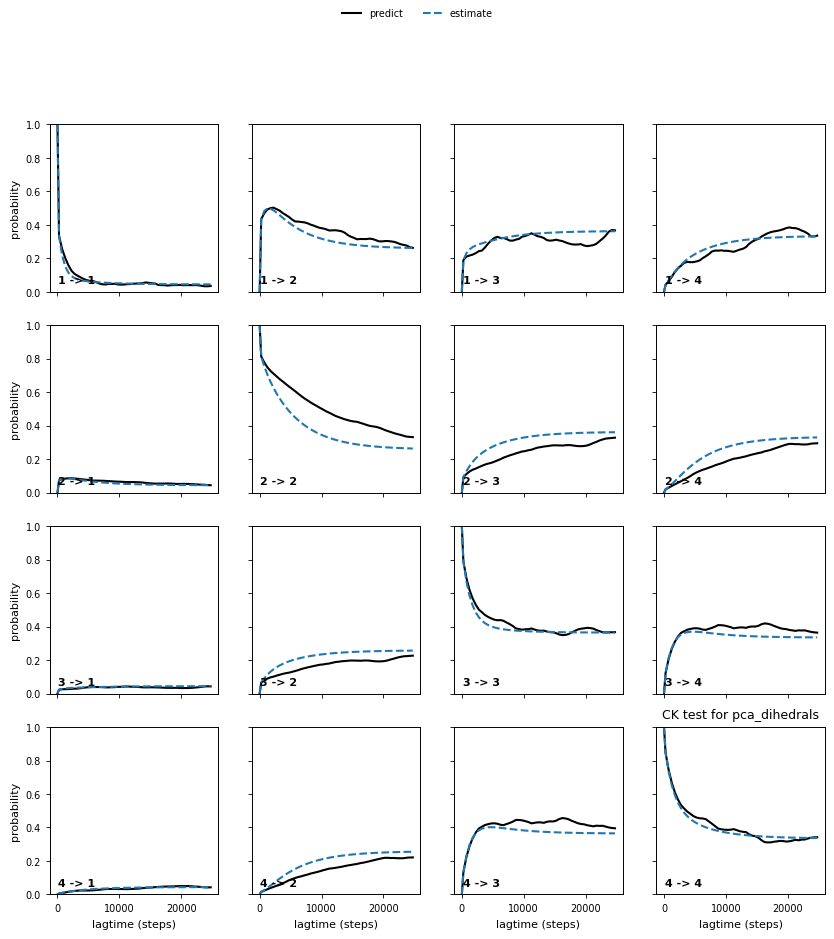
\includegraphics[width=0.5\linewidth]{figures/CK_example.png}
\caption{\textbf{Chapman--Kolmogorov test for the pca-dihedrals MSM}. The microstate
model estimated at $\tau = 50$\,ns was lumped into four metastable sets with
PCCA++. Each panel ($i\!\to\!j$) shows the probability of being in set $j$ at
time $k\tau$ given the system started in set $i$. Solid lines: MSMs estimated
independently at each lag; dashed lines: predictions from the $\tau = 50$\,ns
model. Close agreement indicates approximate Markovianity at the chosen lag.}
\label{suppfig:ck}
\end{figure}

% ------------- First eigenvector of all models -------------------------
\begin{figure}[!t]
    \centering
    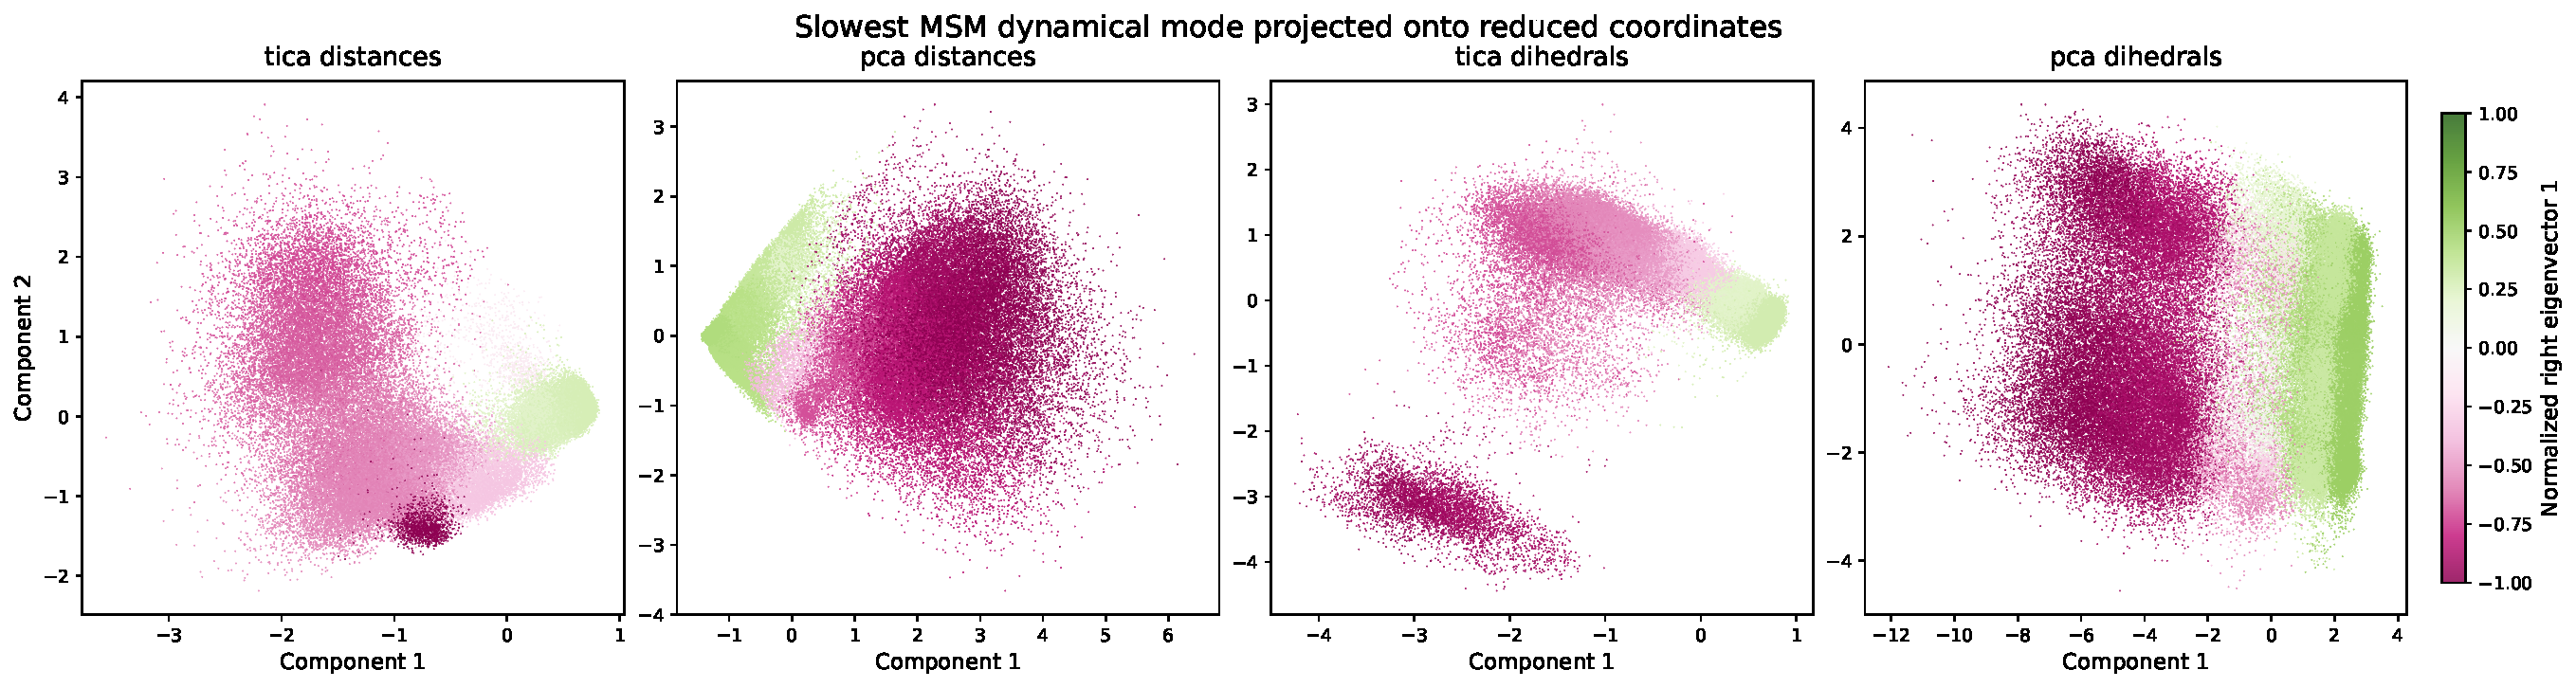
\includegraphics[width=0.5\linewidth]{figures/msm_right_eigenvector_1_projection.pdf}
    \vspace{1em}
    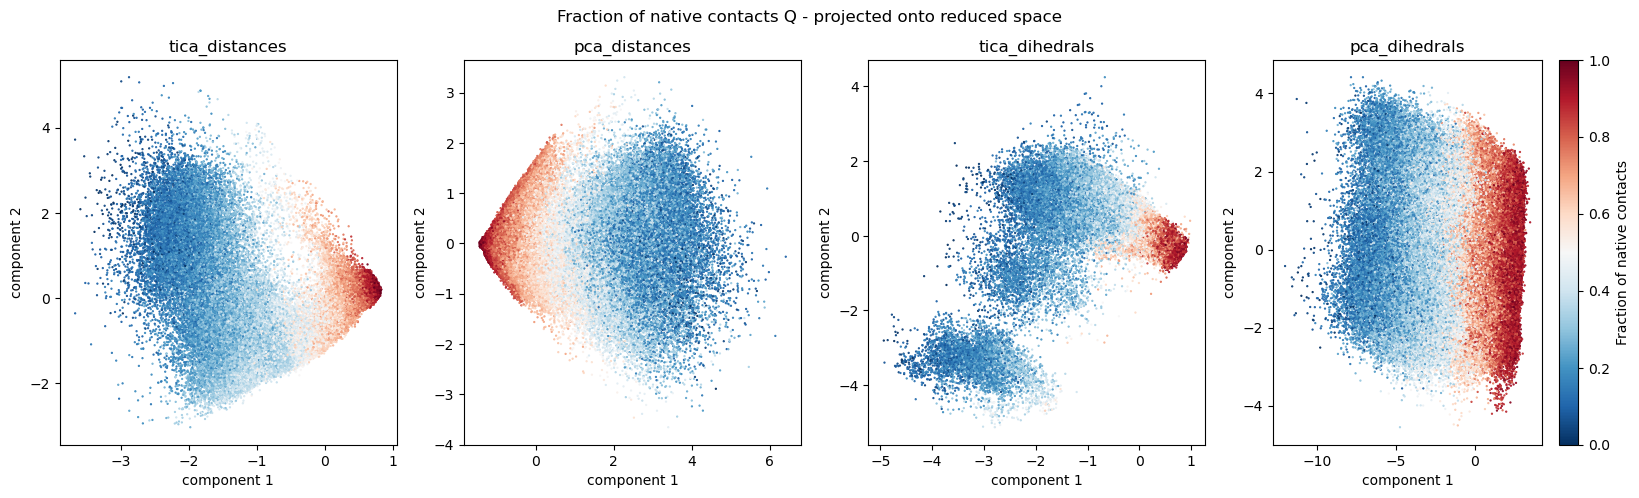
\includegraphics[width=0.5\linewidth]{figures/Q_reduced_projection.png}
    \caption{\small \textbf{Comparison between the slowest MSM relaxation mode and a structural folding descriptor.} 
    Top row: values of the first non-trivial eigenvector projected onto the first two components of the reduced coordinate space.
    Positive and negative components identify regions that exchange probability on the slowest resolved timescale of the Markov model. 
    Bottom row: projection of the fraction of native contacts, Q, onto the same coordinates. 
    The close correspondence between the eigenvector sign pattern and the distribution of $Q$ indicates that the slowest kinetic process 
    captured by the MSM is associated with the folding-unfolding transition.}
    \label{suppfig:first_right_eigenvector}
\end{figure}


\begin{figure*}[ht]
    \centering
    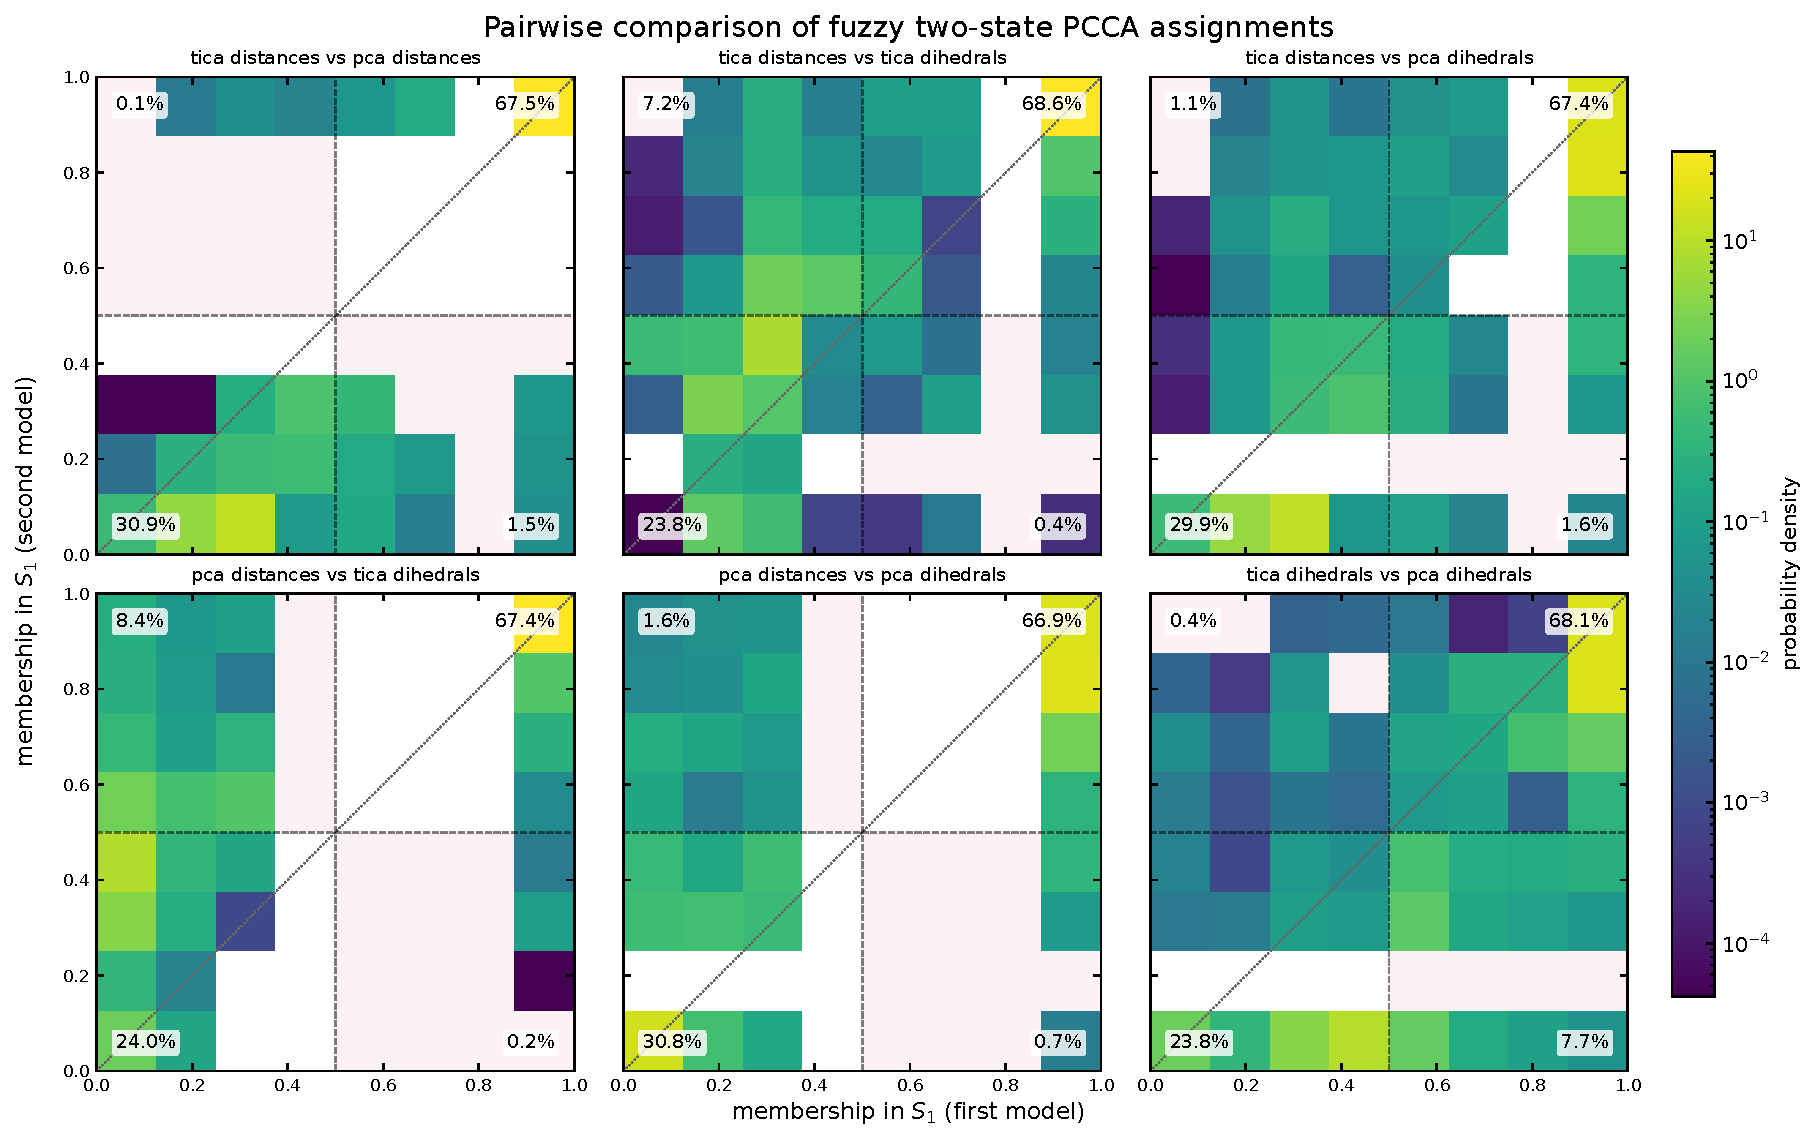
\includegraphics[width=0.7\linewidth]{figures/pairwise_pcca_hist2d.pdf}
    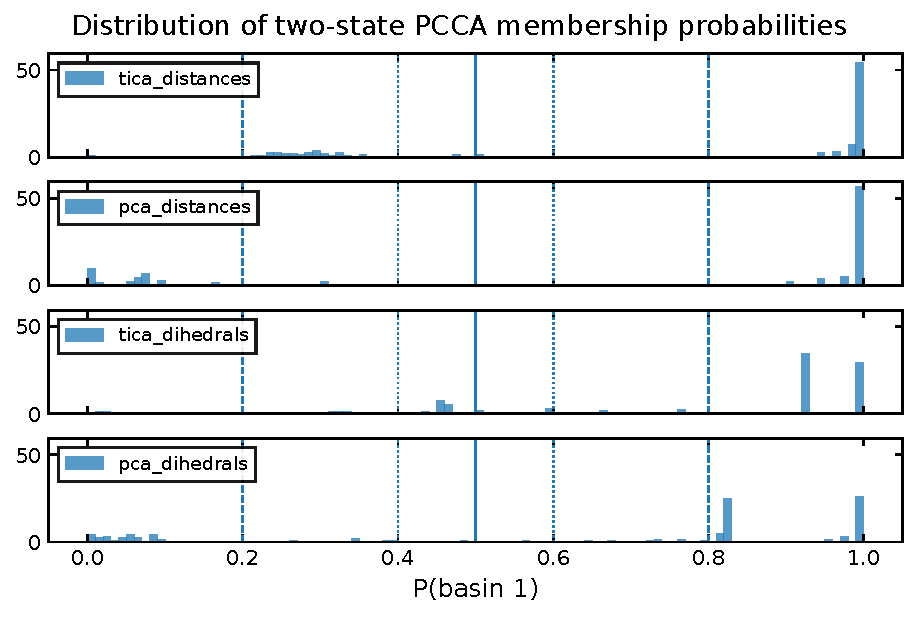
\includegraphics[width = 0.5 \linewidth]{figures/pcca_membership_probability_distributions.pdf}
    \caption{\small \textit{Fuzzy membership probabilities of the trajectory frames to the two macrostates across models. Top: Each panel shows the fuzzy membership probability of each frame in the trajectory to macrostate $S_0$ ($\simeq$ denatured basin) and macrostate $S_1$ ($\simeq$folded basin) for a different model. The models based on distances (tica-distances and pca-distances) show very similar distributions, while the tica-dihedrals model exhibits a broader distribution, particularly for frames assigned to the denatured basin. This indicates that the tica-dihedrals model has more uncertainty in assigning frames to the denatured basin. Bottom: Distribution of the fuzzy membership probability of each frame to macrostate $1$ for the four MSMs. Probabilities close to $0$ or $1$ correspond to frames that are confidently assigned to a single macrostate. }}
    \label{suppfig:fuzzy_memberships_models}
\end{figure*}


% ----- Helix content in the consensus vs other
\begin{figure}[h!]
    \centering
    
\includegraphics[width = 0.8\linewidth]{figures/twostate_helix_differences.pdf}
    \caption{\small \textbf{Helix content in the consensus $S_1$ frames:} Distribution of distances for all intra-helical contacts in the consensus folded ensemble (\(S_1\), blue) and in all other frames (orange). The black squares marks the distance observed in the crystal structure PDB 2F4K. Although helical contacts are generally more compact within \(S_1\), their distributions overlap substantially with those of the remaining frames, indicating that significant helical structure is present both inside and outside the folded basin. }
    \label{suppfig:twostate_helix}
\end{figure}
\begin{figure}[h!]
    \centering
    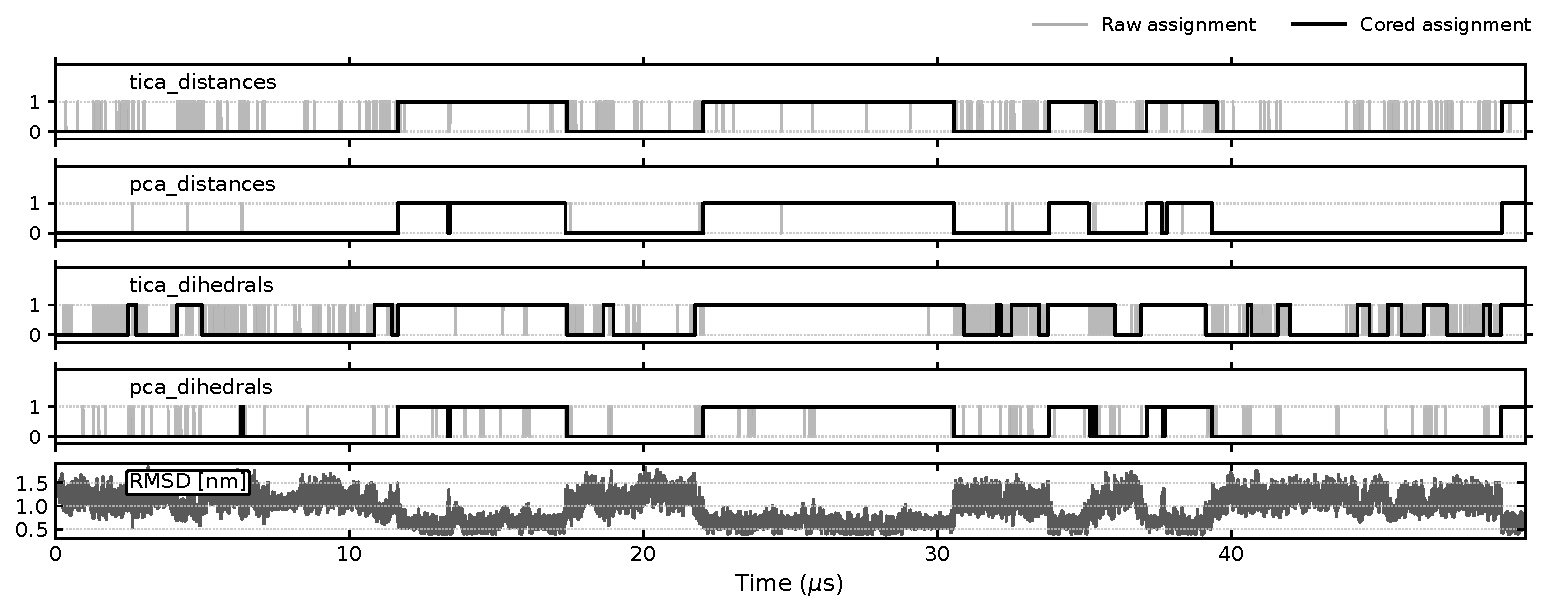
\includegraphics[width=0.8\linewidth]{figures/two_state_raw_vs_cored_assignments.pdf}
\caption{\small
\textbf{Comparison of raw and filtered macrostate trajectories for the two-state PCCA++ models.}
For each MSM, the grey trace shows the instantaneous hard assignment of each frame, while the black trace shows the filtered assignment obtained by removing transitions that persist for less than one Markov lag time ($\tau = 50\,\mathrm{ns}$). The RMSD time series is shown at the bottom for reference. This filtering suppresses rapid recrossings near the state boundary and highlights the long-lived folded and unfolded episodes underlying the dynamics. Only the first $\simeq 50\,\mu s$ of the trajectory are shown.
}
    \label{suppfig:twostate_traj}
\end{figure}
\begin{table}[h!]
    \begin{tabular}{lccccc}
        \hline
        Model
        & $P(S_0)$
        & $P(S_1)$
        & $\langle t_0\rangle$ ($\mu$s)
        & $\langle t_1\rangle$ ($\mu$s)
        & $\Delta G_{1-0}$ (kcal mol$^{-1}$) \\
        \hline
        tICA distances  & 0.230 & 0.770 & 1.591 & 5.312 & -0.863 \\
        PCA distances   & 0.303 & 0.697 & 1.933 & 4.446 & -0.596 \\
        tICA dihedrals  & 0.218 & 0.782 & 1.471 & 5.286 & -0.915 \\
        PCA dihedrals   & 0.358 & 0.642 & 1.407 & 2.520 & -0.417 \\
        \hline
    \end{tabular}
\caption{\small
\textbf{Thermodynamic and kinetic properties estimated from two-state Markov Models:}
Stationary populations, mean residence times, and relative free energies obtained from the two-state Markov model induced by the PCCA++ coarse graining of each MSM. Mean residence times were computed as $\langle t_i\rangle=\tau/(1-T_{ii})$, where $T$ denotes the coarse-grained transition matrix and $\tau$ the MSM lag time. Relative free energies were calculated as $\Delta G_{1-0}=-k_{\mathrm B}T\ln[P(S_1)/P(S_0)]$ at $T=360$ K.
}
    \label{supptab:pcca_model_estimates}
\end{table}
% ------------- Three state tica-dihedrals -------------------------
\begin{figure*}[ht]
\centering
    %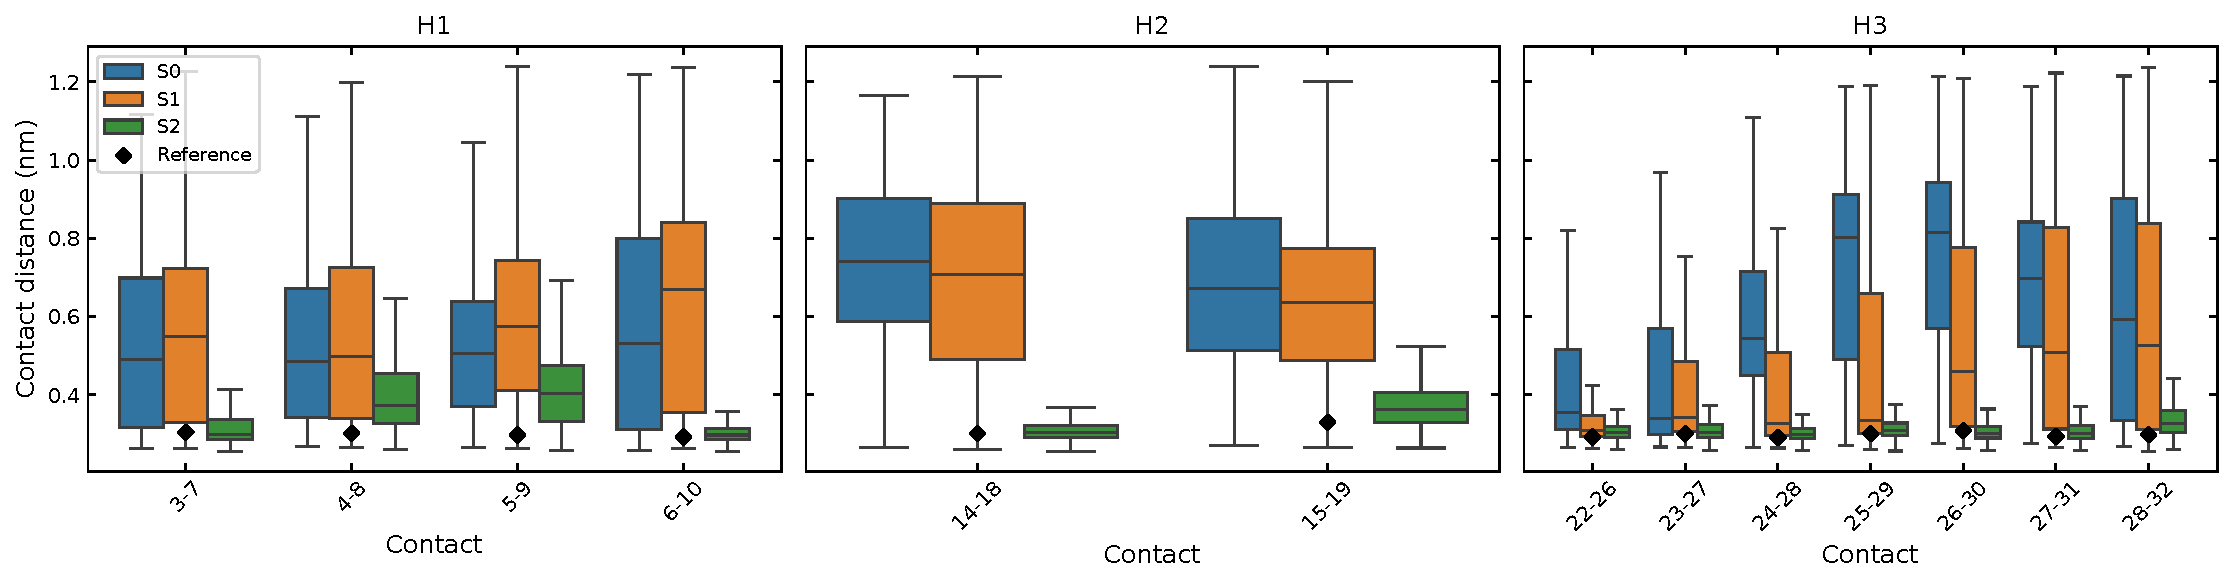
\includegraphics[width=0.7\linewidth]{figures/threestate_dihedrals_helix_differences.pdf}
    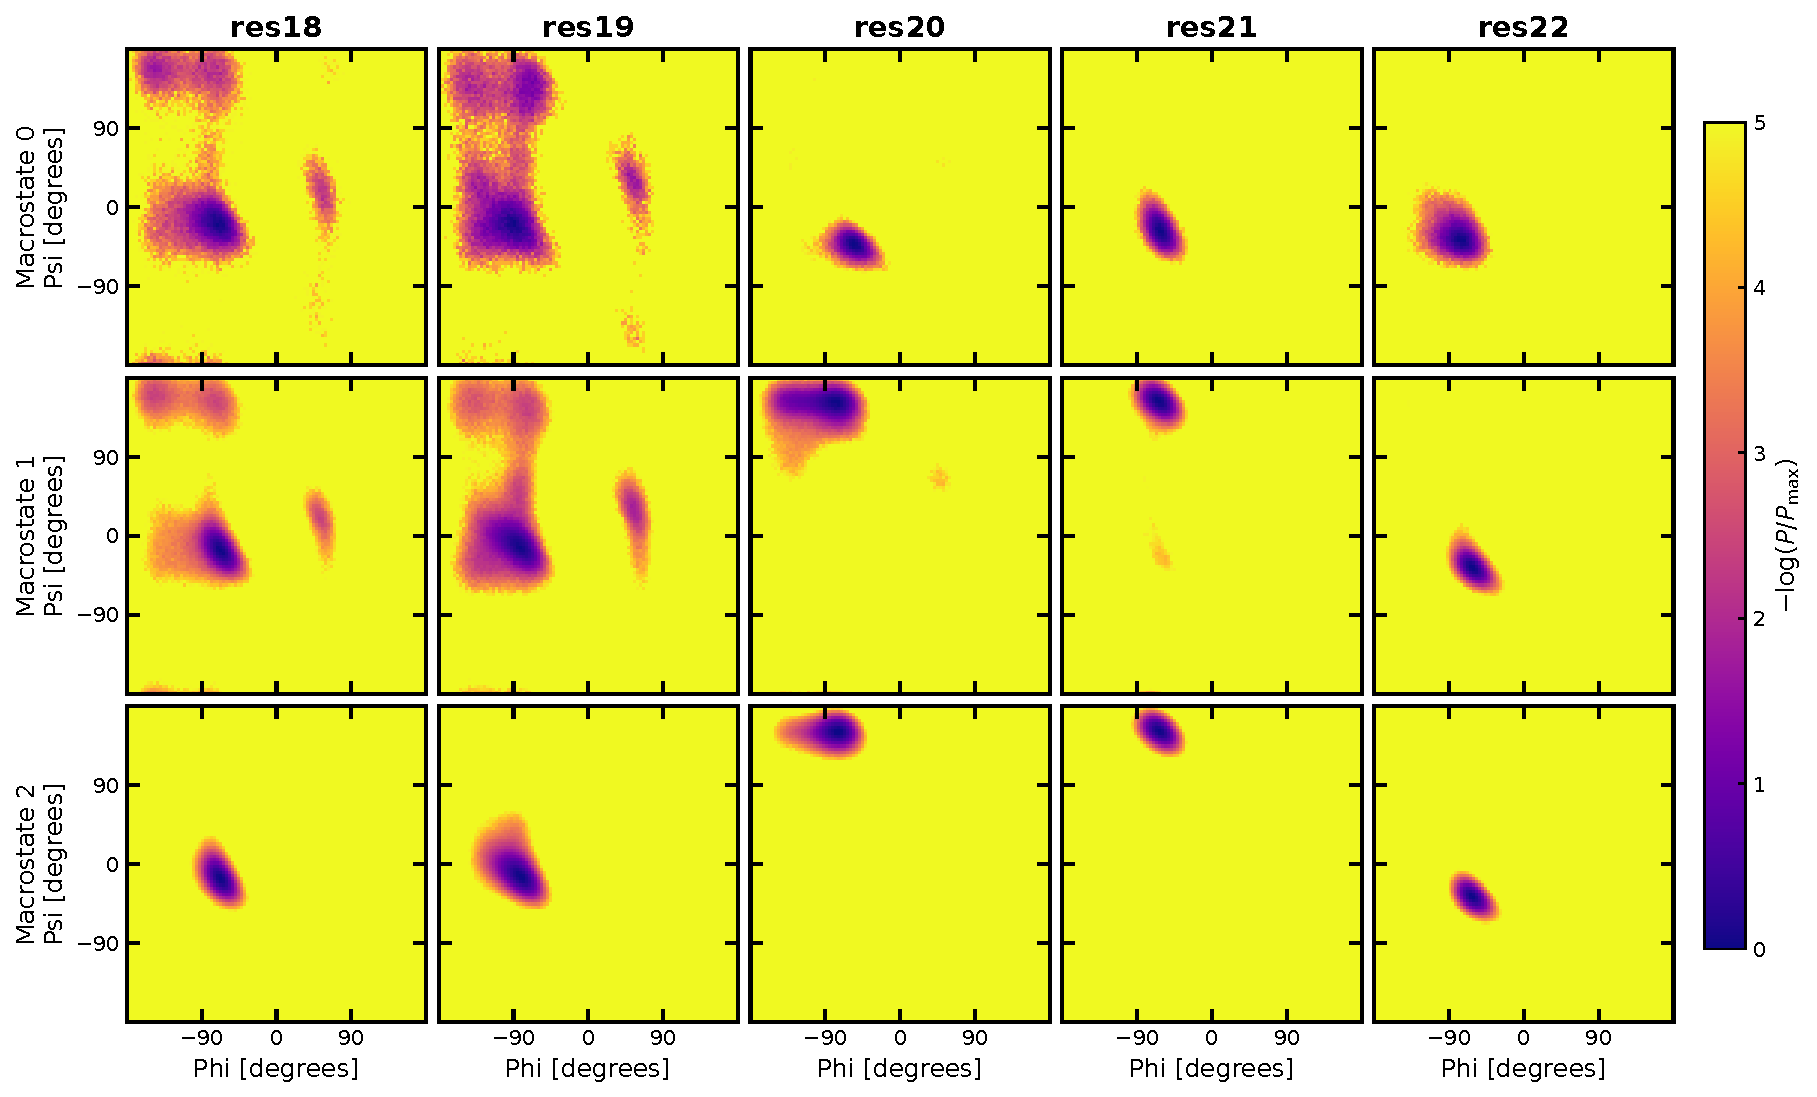
\includegraphics[width=0.4\linewidth]{figures/dihedrals_ramachandran_macrostate_comparison.pdf}
    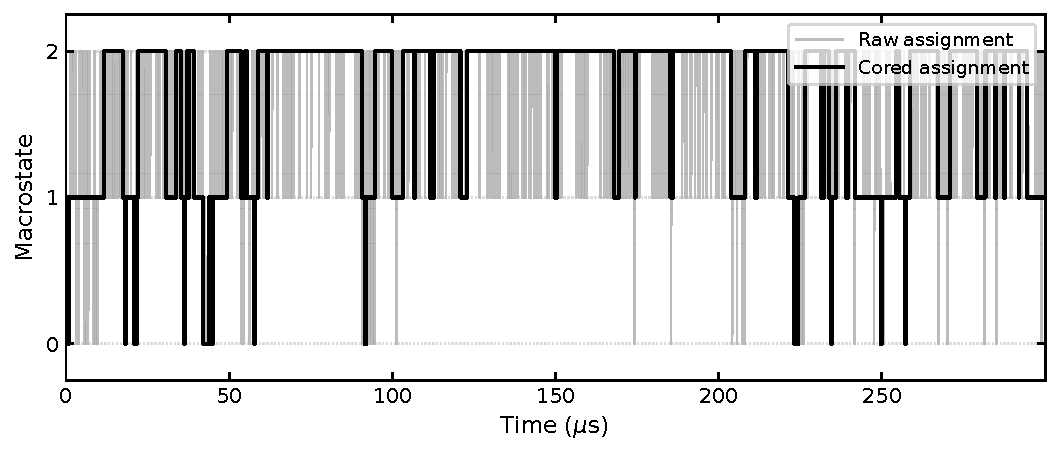
\includegraphics[width=0.4\linewidth]{figures/tica_dihedrals_3_pcca_coring_trajectory.pdf}
    \caption{\small {\textbf{Structural caracterization of the 3-state PCCA macrostates for the tica-dihedrals model:} Top: ($\phi, \psi$) distribution of the residues $18-22$ in the three macrostates $S_0, S_1, S_2$.
    Bottom: trajectory of the three-state PCCA++ model for tICA-dihedrals, with hard assignations and cored assignations (transitions are counted if they remain in the destination for at least one markov step, which is $\tau = 50\,ns$).}}
    \label{suppfig:threestate_tica_dihedrals}
\end{figure*}


% ---------- Manual analysis of the dihedral model
\begin{figure}[h!]
    \centering
    %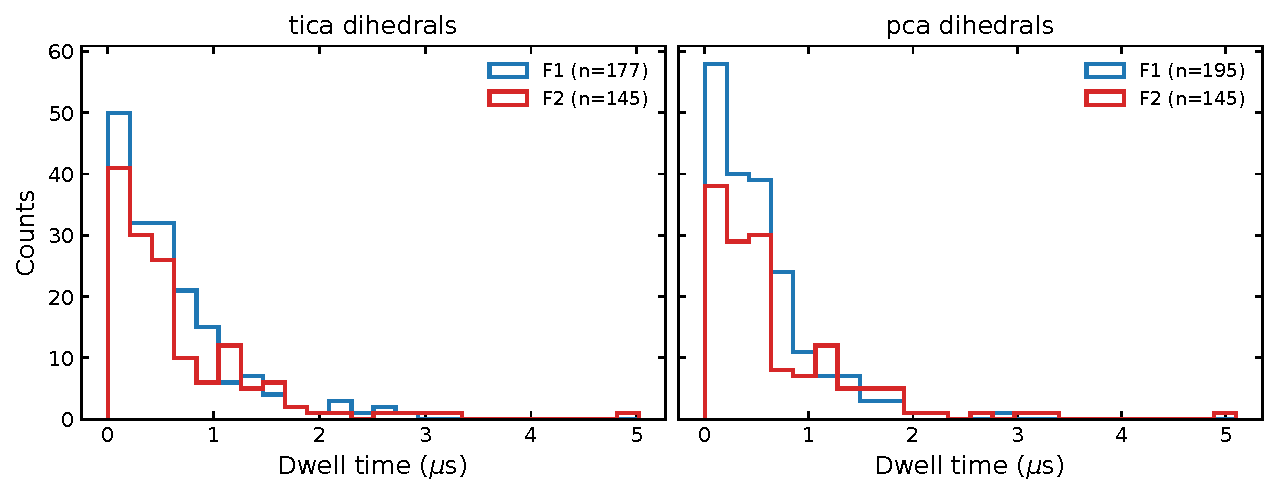
\includegraphics[width=0.45\linewidth]{figures/f1_f2_dwell_time_histograms.pdf}
    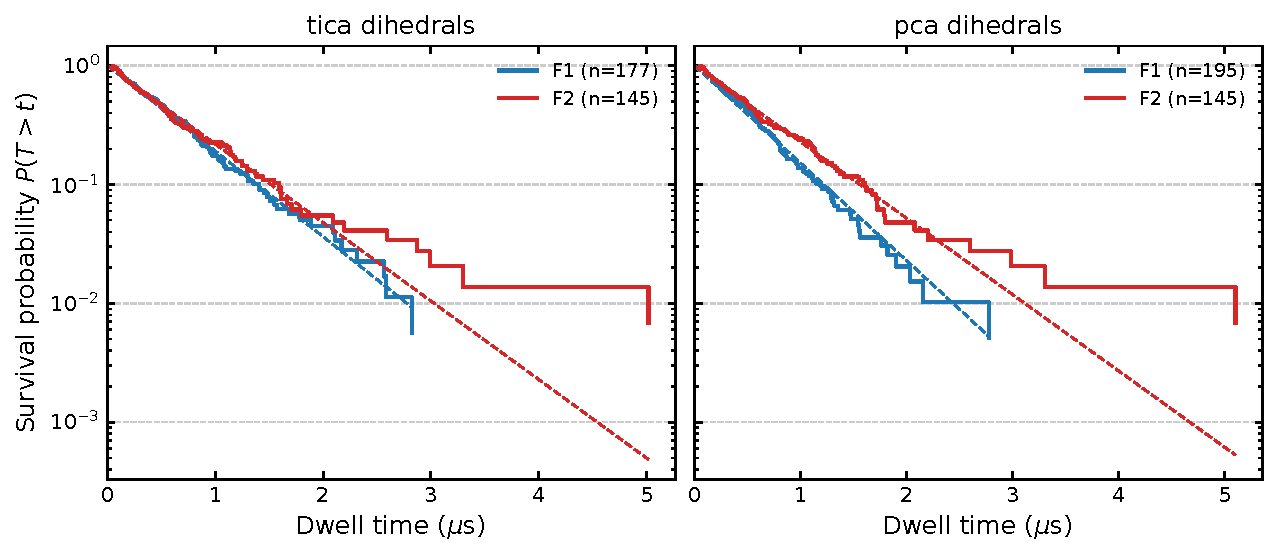
\includegraphics[width=0.8\linewidth]{figures/f1_f2_dwell_time_survival.pdf}
    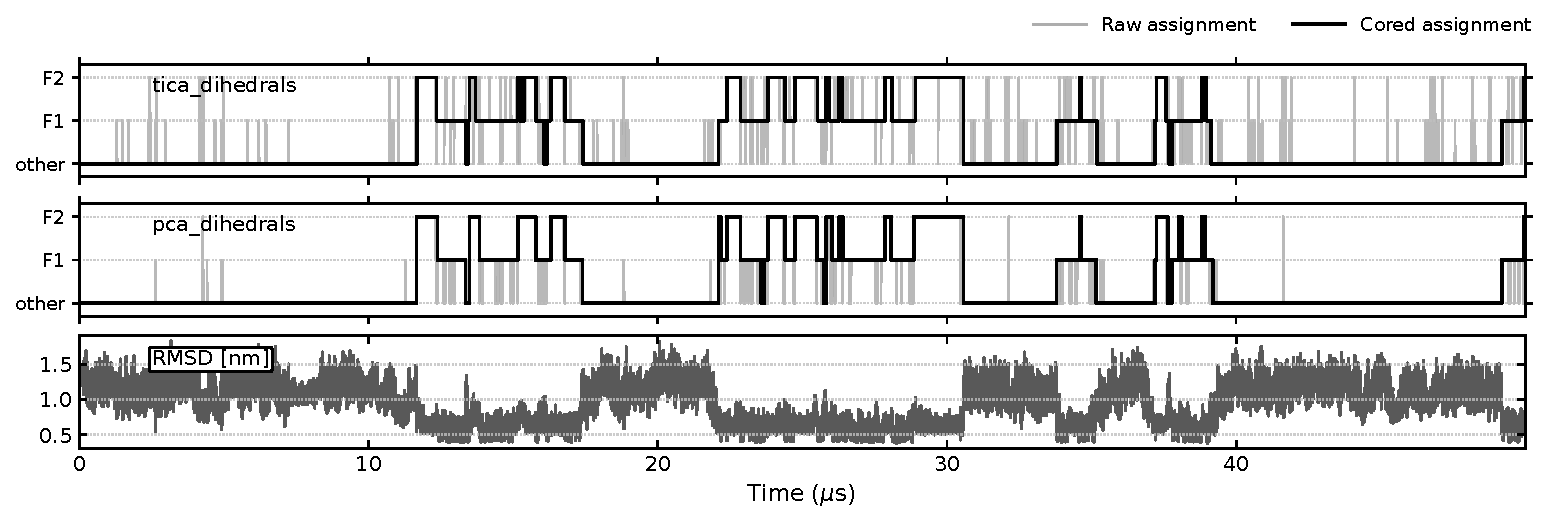
\includegraphics[width = \linewidth]{figures/f1_f2_raw_vs_cored_assignments.pdf}
    \caption{Manual analysis of dihedral-resolved substates.}
    \label{suppfig:f1f2_figure}
\end{figure}


\begin{table}[h!]
\begin{tabular}{llrrrr}
\hline
Model & State & $N_{\mathrm{visits}}$ & Mean [$\mu$s] & Median [$\mu$s] & Population \\
\hline
tica\_dihedrals & F1 & 177 & 0.603 & 0.463 & 0.350 \\
tica\_dihedrals & F2 & 145 & 0.658 & 0.435 & 0.313 \\
pca\_dihedrals & F1 & 195 & 0.529 & 0.412 & 0.338 \\
pca\_dihedrals & F2 & 145 & 0.676 & 0.480 & 0.321 \\
\hline
\end{tabular}
\caption{Dwell times in the folded sub-basins $F_1$ and $F_2$, computed from the cored microstate trajectory of each dihedral model. $N_{\mathrm{visits}}$ is the number of continuous visits to the sub-basin, and the population is the fraction of cored frames assigned to it.}
\label{tab:f1_f2_dwell_times}
\end{table}